\section{Preventivo} 
	\subsection{Introduzione}
		A fronte della pianificazione sono state decise per ogni periodo quante ore ogni componente del gruppo dovrà svolgere per ruolo.
		Per favorire la rotazione dei ruoli sarà possibile che alcuni membri in una singolo periodo svolgano diversi ruoli. \\
		Nelle tabelle e in alcuni grafici si farà uso delle abbreviazioni seguenti per indicare i ruoli:
		\begin{itemize} 
			\item \textbf{RE}: Responsabile;
			\item \textbf{AM}: Amministratore;
			\item \textbf{AN}: Analista;
			\item \textbf{PG}: Progettista;
			\item \textbf{PR}: Programmatore;
			\item \textbf{VR}: Verificatore.
		\end{itemize}
		
	\newpage	
	\subsection{Periodo non rendicontato}
		
		\subsubsection{Periodo di analisi e management}
		
			\paragraph{Suddivisione del lavoro}
			Nella seguente tabella è descritta la divisione del lavoro nel periodo di analisi e management:
			\begin{tabella}{!{\VRule}c!{\VRule}c!{\VRule}c!{\VRule}c!{\VRule}c!{\VRule}c!{\VRule}c!{\VRule}c!{\VRule}}
				
				\intestazioneeightcol{Nome}{RE}{AM}{AN}{PG}{PR}{VR}{Ore totali}
				
				Viviana Alessio & 12 & 2 & - & - & - & 8 & 22 \\
				Enrico Bellio & - & - & 15 & - & - & 7 & 22 \\
				Matteo Franco & - & 14 & - & - & - & 8 & 22 \\
				Andrea Grendene & - & - & 20 & - & - & 3 & 23 \\
				Tommaso Panozzo & - & 6 & 15 & - & - & 3 & 24 \\
				Luca Soldera  & - & 14 & - & - & - & 8 & 22 \\
				\hline
				\textbf{Ore totali} & \textbf{12} & \textbf{36} & \textbf{50} & \textbf{-} & \textbf{-} & \textbf{37} & \textbf{135} \\
				
				\hiderowcolors
				\caption{Ore per componente - Periodo di analisi e management}
				
			\end{tabella}
			
			Vengono esposti visivamente i dati riportati in tabella attraverso il seguente istogramma:
			\ist{img/istogrammiOre/istA}{Istogramma ruoli - periodo di analisi e management}
			\newpage
			
			\paragraph{Prospetto economico}
			I costi di questo periodo non vengono rendicontati al Proponente. Nella seguente tabella sono riportati i costi relativi al periodo di analisi e management: 
			\begin{tabella}{!{\VRule}c!{\VRule}c!{\VRule}c!{\VRule}}
				\intestazionethreecol{Ruolo}{Ore}{Costo}
				
				Responsabile & 12 & 360\euro \\
				Amministratore & 36 & 720\euro \\
				Analista & 50 & 1250\euro \\
				Progettista & - & - \\
				Programmatore & - & - \\
				Verificatore & 37 & 555\euro \\
				\hline
				\textbf{Totale} & \textbf{135} & \textbf{2885\euro} \\
				\hiderowcolors
				\caption{Ore per ruolo - Periodo di analisi e management}
			\end{tabella}
			
			\torta{img/percSoldi/percSoldiA.png}{Percentuale di costo per ruolo sul totale - Periodo di analisi e management}	
			\torta{img/percOre/PercentualeOreFaseA.png}{Percentuale di ore per ruolo sul totale - Periodo di analisi e management}
			\newpage
			
	\subsection{Periodi rendicontati}
	
		\subsubsection{Periodo di consolidamento dei requisiti}
			\paragraph{Suddivisione del lavoro}
			Nella seguente tabella è descritta la divisione del lavoro nella periodo di consolidamento dei requisiti: \\ \\
			\begin{tabella}{!{\VRule}c!{\VRule}c!{\VRule}c!{\VRule}c!{\VRule}c!{\VRule}c!{\VRule}c!{\VRule}c!{\VRule}}
				
				\intestazioneeightcol{Nome}{RE}{AM}{AN}{PG}{PR}{VR}{Ore totali}
				
				Viviana Alessio & - & - & 12 & - & - & - & 12 \\
				Enrico Bellio & - & - & - & - & - & 10 & 10 \\
				Matteo Franco & - & - & 10 & - & - & - & 10 \\
				Andrea Grendene & - & 3 & - & - & - & 7 & 10 \\
				Tommaso Panozzo & - & 5 & 3 & - & - & - & 8 \\
				Luca Soldera  & 5 & - & 5 & - & - & - & 10 \\
				\hline
				\textbf{Ore totali} & \textbf{5} & \textbf{8} & \textbf{30} & \textbf{-} & \textbf{-} & \textbf{17} & \textbf{60} \\
				
				\hiderowcolors
				\caption{Ore per componente - Periodo di consolidamento dei requisiti}
				
			\end{tabella}
			
			
			\ist{img/istogrammiOre/istAD}{Istogramma ruoli - Periodo di consolidamento dei requisiti}
			\newpage
			
			\paragraph{Prospetto economico}
			Nella seguente tabella sono riportati i costi relativi alla periodo di consolidamento dei requisiti da rendicontare al Proponente: 
			\begin{tabella}{!{\VRule}c!{\VRule}c!{\VRule}c!{\VRule}}
				\intestazionethreecol{Ruolo}{Ore}{Costo}
				
				Responsabile & 5 & 150\euro \\
				Amministratore & 8 & 160\euro \\
				Analista & 30 & 750\euro \\
				Progettista & - & - \\
				Programmatore & - & - \\
				Verificatore & 17 & 255\euro \\
				\hline
				\textbf{Totale} & \textbf{60} & \textbf{1315\euro} \\
				\hiderowcolors
				\caption{Ore per ruolo - Periodo di consolidamento dei requisiti}
				\end{tabella}	
			
			\torta{img/percSoldi/percSoldiAD.png}{Percentuale di costo per ruolo sul totale - Periodo di consolidamento dei requisiti}	
			\torta{img/percOre/PercentualeOreFaseAD.png}{Percentuale di ore per ruolo sul totale - Periodo di consolidamento dei requisiti}
		\newpage
		
		\subsubsection{Periodo di progettazione architetturale}
			\paragraph{Suddivisione del lavoro}
			Nella seguente tabella è descritta la divisione del lavoro nella periodo di progettazione architetturale:
			\begin{tabella}{!{\VRule}c!{\VRule}c!{\VRule}c!{\VRule}c!{\VRule}c!{\VRule}c!{\VRule}c!{\VRule}c!{\VRule}}
				
				\intestazioneeightcol{Nome}{RE}{AM}{AN}{PG}{PR}{VR}{Ore totali}
				
				Viviana Alessio & - & - & - & 23 & - & 12 & 35 \\
				Enrico Bellio & - & 5 & 10 & - & - & 18 & 33 \\
				Matteo Franco & 10 & - & - & 23 & - & - & 33 \\
				Andrea Grendene & - & - & - & 20 & - & 15 & 35 \\
				Tommaso Panozzo & - & 5 & 10 & - & - & 20 & 35 \\
				Luca Soldera  & - & - & - & 25 & - & 10 & 35 \\
				\hline
				\textbf{Ore totali} & \textbf{10} & \textbf{10} & \textbf{20} & \textbf{91} & \textbf{-} & \textbf{75} & \textbf{206} \\
				
				\hiderowcolors
				\caption{Ore per componente - Periodo di progettazione architetturale}
				
			\end{tabella}
			
			\ist{img/istogrammiOre/istPA}{Istogramma ruoli - Periodo di progettazione architetturale}
			\newpage
			
			\paragraph{Prospetto economico}
			Nella seguente tabella sono riportati i costi relativi alla periodo di progettazione architetturale da rendicontare al Proponente: 
			\begin{tabella}{!{\VRule}c!{\VRule}c!{\VRule}c!{\VRule}}
				\intestazionethreecol{Ruolo}{Ore}{Costo}
				
				Responsabile & 10 & 300\euro \\
				Amministratore & 10 & 200\euro \\
				Analista & 20 & 500\euro \\
				Progettista & 91 & 2002\euro \\
				Programmatore & - & - \\
				Verificatore & 75 & 1125\euro \\
				\hline
				\textbf{Totale} & \textbf{206} & \textbf{4127\euro} \\
				\hiderowcolors
				\caption{Ore per ruolo - Periodo di progettazione architetturale}
				\end{tabella}
			
			\torta{img/percSoldi/percSoldiPA.png}{Percentuale di costo per ruolo sul totale - Periodo di progettazione architetturale}	
			\torta{img/percOre/PercentualeOreFasePA.png}{Percentuale di ore per ruolo sul totale - Periodo di progettazione architetturale}
			\newpage
		
		\subsubsection{Periodo di progettazione di dettaglio e codifica}
			\paragraph{Suddivisione del lavoro}
			Nella seguente tabella è descritta la divisione del lavoro nella periodo di progettazione di dettaglio e codifica:
			\begin{tabella}{!{\VRule}c!{\VRule}c!{\VRule}c!{\VRule}c!{\VRule}c!{\VRule}c!{\VRule}c!{\VRule}c!{\VRule}}
				
				\intestazioneeightcol{Nome}{RE}{AM}{AN}{PG}{PR}{VR}{Ore totali}
				
				Viviana Alessio & - & - & - & - & 20 & 15 & 35 \\
				Enrico Bellio & - & - & - & 20 & 10 & 5 & 35 \\
				Matteo Franco & - & - & 6 & 4 & 10 & 15 & 35 \\
				Andrea Grendene & - & - & - & - & 25 & 10 & 35 \\
				Tommaso Panozzo & 10 & - & - & 11 & 7 & 7 & 35 \\
				Luca Soldera  & - & 5 & 3 & 10 & 3 & 13 & 34 \\
				\hline
				\textbf{Ore totali} & \textbf{10} & \textbf{5} & \textbf{9} & \textbf{45} & \textbf{75} & \textbf{65} & \textbf{209} \\
				
				\hiderowcolors
				\caption{Ore per componente - Periodo di progettazione di dettaglio e codifica}
				
			\end{tabella}
			
			\ist{img/istogrammiOre/istPDC}{Istogramma ruoli - Periodo di progettazione di dettaglio e codifica}
			\newpage
			
			\paragraph{Prospetto economico}
			Nella seguente tabella sono riportati i costi relativi alla periodo di progettazione di dettaglio e codifica da rendicontare al Proponente: 
			\begin{tabella}{!{\VRule}c!{\VRule}c!{\VRule}c!{\VRule}}
				\intestazionethreecol{Ruolo}{Ore}{Costo}
				
				Responsabile & 10 & 300\euro \\
				Amministratore & 5 & 100\euro \\
				Analista & 9 & 225\euro \\
				Progettista & 45 & 990\euro \\
				Programmatore & 75 & 1125\euro \\
				Verificatore & 65 & 975\euro \\
				\hline
				\textbf{Totale} & \textbf{209} & \textbf{3715\euro} \\
				\hiderowcolors
				\caption{Ore per ruolo - Periodo di progettazione di dettaglio e codifica}
			\end{tabella}	

			\begin{figure}[!h]
				\centering
				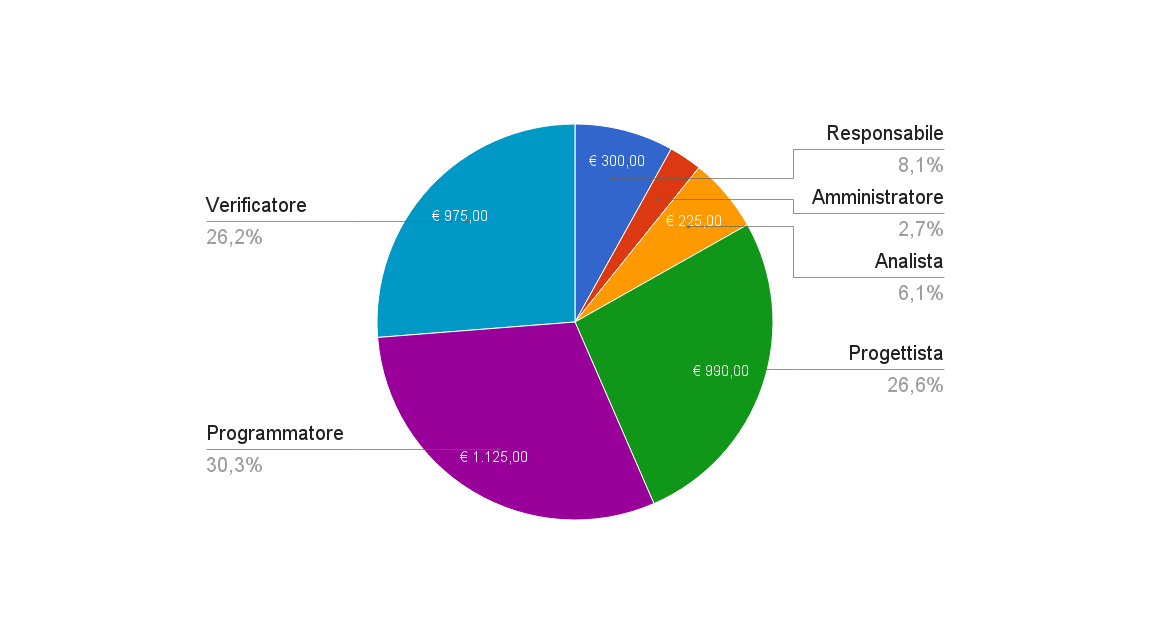
\includegraphics[height=6.3cm, width=11.4cm]{img/percSoldi/percSoldiPDC.png} 
				\caption{Percentuale di costo per ruolo sul totale - Periodo di progettazione di dettaglio e codifica}
			\end{figure}
			
			
			\begin{figure}[!h]
				\centering
				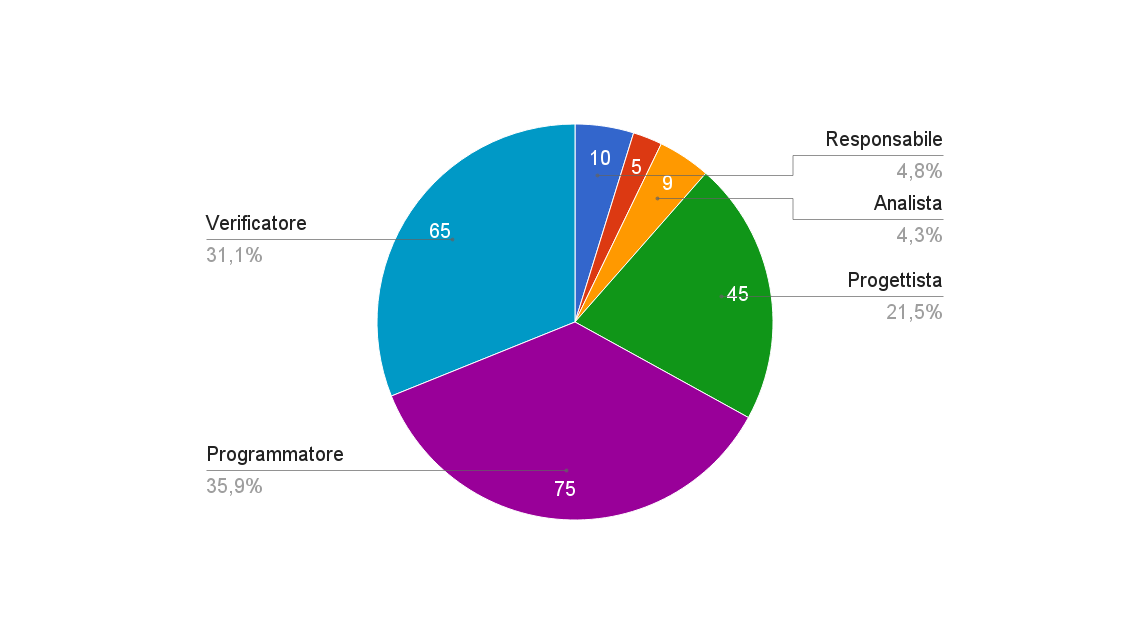
\includegraphics[height=6.3cm, width=11.4cm]{img/percOre/PercentualeOreFasePDC.png} 
				\caption{Percentuale di ore per ruolo - Periodo di progettazione di dettaglio e codifica}
			\end{figure}
			
			\newpage	
		
		\subsubsection{Periodo di codifica dei requisiti desiderabili e opzionali}	
			\paragraph{Suddivisione del lavoro}
			Nella seguente tabella è descritta la divisione del lavoro nella periodo di codifica dei requisiti desiderabili e opzionali:
			\begin{tabella}{!{\VRule}c!{\VRule}c!{\VRule}c!{\VRule}c!{\VRule}c!{\VRule}c!{\VRule}c!{\VRule}c!{\VRule}}
				
				\intestazioneeightcol{Nome}{RE}{AM}{AN}{PG}{PR}{VR}{Ore totali}
				
				Viviana Alessio & - & 3 & 2 & - & - & 5 & 10 \\
				Enrico Bellio & 3 & - & - & 6 & - & 3 & 12 \\
				Matteo Franco & - & - & - & 3 & 10 & - & 13 \\
				Andrea Grendene & - & - & - & - & - & 11 & 11 \\
				Tommaso Panozzo & - & - & - & 5 & 4 & 2 & 11 \\
				Luca Soldera  & - & - & - & - & 12 & - & 12 \\
				\hline
				\textbf{Ore totali} & \textbf{3} & \textbf{3} & \textbf{2} & \textbf{14} & \textbf{26} & \textbf{21} & \textbf{69} \\
				
				\hiderowcolors
				\caption{Ore per componente - Periodo di codifica dei requisiti desiderabili e opzionali}
				
			\end{tabella}
			
			\ist{img/istogrammiOre/istRD}{Istogramma ruoli - Periodo di codifica dei requisiti desiderabili e opzionali}

			\newpage
			
			\paragraph{Prospetto economico}
			Nella seguente tabella sono riportati i costi relativi alla periodo di codifica dei requisiti desiderabili e opzionali da rendicontare al Proponente: 
			\begin{tabella}{!{\VRule}c!{\VRule}c!{\VRule}c!{\VRule}}
				\intestazionethreecol{Ruolo}{Ore}{Costo}
				
				Responsabile & 3 & 90\euro \\
				Amministratore & 3 & 60\euro \\
				Analista & 2 & 50\euro \\
				Progettista & 14 & 308\euro \\
				Programmatore & 26 & 390\euro \\
				Verificatore & 21 & 315\euro \\
				\hline
				\textbf{Totale} & \textbf{69} & \textbf{1213\euro} \\
				\hiderowcolors
				\caption{Ore per ruolo - Periodo di codifica dei requisiti desiderabili e opzionali}
			\end{tabella}
			
			\torta{img/percSoldi/percSoldiRD.png}{Percentuale di costo per ruolo sul totale - Periodo di codifica dei requisiti desiderabili e opzionali}	
			\torta{img/percOre/PercentualeOreFaseRD.png}{Percentuale di ore per ruolo sul totale - Periodo di codifica dei requisiti desiderabili e opzionali}
			\newpage
		
		\subsubsection{Periodo di validazione e collaudo}
			\paragraph{Suddivisione del lavoro}
			Nella seguente tabella è descritta la divisione del lavoro nel periodo di validazione e collaudo:
			\begin{tabella}{!{\VRule}c!{\VRule}c!{\VRule}c!{\VRule}c!{\VRule}c!{\VRule}c!{\VRule}c!{\VRule}c!{\VRule}}
				
				\intestazioneeightcol{Nome}{RE}{AM}{AN}{PG}{PR}{VR}{Ore totali}
				
				Viviana Alessio & - & 3 & 2 & - & - & 5 & 10 \\
				Enrico Bellio & - & 5 & - & - & - & 7 & 12 \\
				Matteo Franco & - & - & - & 3 & - & 8 & 11 \\
				Andrea Grendene & 5 & - & - & - & 6 & - & 11 \\
				Tommaso Panozzo & - & - & - & 5 & 5 & 3 & 13 \\
				Luca Soldera  & - & - & - & - & 5 & 6 & 11 \\
				\hline
				\textbf{Ore totali} & \textbf{5} & \textbf{8} & \textbf{2} & \textbf{8} & \textbf{16} & \textbf{29} & \textbf{68} \\
				
				\hiderowcolors
				\caption{Ore per componente - Periodo di validazione e collaudo}
				
			\end{tabella}

			
			\ist{img/istogrammiOre/istV}{Istogramma ruoli - Periodo di validazione e collaudo}	
			\newpage
			
			\paragraph{Prospetto economico}
			Nella seguente tabella sono riportati i costi relativi alla periodo di validazione e collaudo da rendicontare al Proponente: 
			\begin{tabella}{!{\VRule}c!{\VRule}c!{\VRule}c!{\VRule}}
				\intestazionethreecol{Ruolo}{Ore}{Costo}
				
				Responsabile & 5 & 150\euro \\
				Amministratore & 8 & 160\euro \\
				Analista & 2 & 50\euro \\
				Progettista & 8 & 176\euro \\
				Programmatore & 16 & 240\euro \\
				Verificatore & 29 & 435\euro \\
				\hline
				\textbf{Totale} & \textbf{68} & \textbf{1211\euro} \\
				\hiderowcolors
				\caption{Ore per ruolo - Periodo di validazione e collaudo}
			\end{tabella}
			
			\torta{img/percSoldi/percSoldiV.png}{Percentuale di costo per ruolo sul totale - Periodo di validazione e collaudo}	
			\torta{img/percOre/PercentualeOreFaseV.png}{Percentuale di ore per ruolo sul totale - Periodo di validazione e collaudo}
			\newpage
			
	\subsection{Riepilogo}
		\subsubsection{Ore investite}
		Di seguito un resoconto delle ore investite nel periodo non rendicontato.
		
		\begin{tabella}{!{\VRule}c!{\VRule}c!{\VRule}c!{\VRule}c!{\VRule}c!{\VRule}c!{\VRule}c!{\VRule}c!{\VRule}}
			
			\intestazioneeightcol{Nome}{RE}{AM}{AN}{PG}{PR}{VR}{Ore totali}
			
			Viviana Alessio & 12 & 2 & - & - & - & 8 & 22 \\
			Enrico Bellio & - & - & 15 & - & - & 7 & 22 \\
			Matteo Franco & - & 14 & - & - & - & 8 & 22 \\
			Andrea Grendene & - & - & 20 & - & - & 3 & 23 \\
			Tommaso Panozzo & - & 6 & 15 & - & - & 3 & 24 \\
			Luca Soldera  & - & 14 & - & - & - & 8 & 22 \\
			\hline
			\textbf{Ore totali} & \textbf{12} & \textbf{36} & \textbf{50} & \textbf{-} & \textbf{-} & \textbf{37} & \textbf{135} \\
			
			\hiderowcolors
			\caption{Ore per componente - Periodo non rendicontata}
			
		\end{tabella}
		
		\ist{img/istogrammiOre/istA}{Istogramma ruoli - Periodo non rendicontato}
		\newpage
		
		Nella seguente tabella sono riportati i costi totali non rendicontabili al Proponente.
		\begin{tabella}{!{\VRule}c!{\VRule}c!{\VRule}c!{\VRule}}
			\intestazionethreecol{Ruolo}{Ore}{Costo}
			
			Responsabile & 12 & 360\euro \\
			Amministratore & 36 & 720\euro \\
			Analista & 50 & 1250\euro \\
			Progettista & - & - \\
			Programmatore & - & - \\
			Verificatore & 37 & 555\euro \\
			\hline
			\textbf{Totale} & \textbf{135} & \textbf{2885\euro} \\
			\hiderowcolors
			\caption{Ore per ruolo - Periodo non rendicontato}
		\end{tabella}
		
		\torta{img/percSoldi/percSoldiA.png}{Percentuale di costo per ruolo sul totale - Periodo non rendicontato}	
		\torta{img/percOre/PercentualeOreFaseA.png}{Percentuale di ore per ruolo sul totale - Periodo non rendicontato}
		\newpage
		
		\subsubsection{Ore rendicontate}
		Di seguito un resoconto delle ore lavorative delle periodi rendicontati.
		
		\begin{tabella}{!{\VRule}c!{\VRule}c!{\VRule}c!{\VRule}c!{\VRule}c!{\VRule}c!{\VRule}c!{\VRule}c!{\VRule}}
			
			\intestazioneeightcol{Nome}{RE}{AM}{AN}{PG}{PR}{VR}{Ore totali}
			
			Viviana Alessio & - & 6 & 16 & 23 & 20 & 37 & 102 \\
			Enrico Bellio & 3 & 10 & 10 & 26 & 10 & 43 & 102 \\
			Matteo Franco & 10 & - & 16 & 33 & 20 & 23 & 102 \\
			Andrea Grendene & 5 & 3 & - & 20 & 31 & 43 & 102 \\
			Tommaso Panozzo & 10 & 10 & 13 & 21 & 16 & 32 & 102 \\
			Luca Soldera  & 5 & 5 & 8 & 35 & 20 & 29 & 102 \\
			\hline
			\textbf{Ore totali} & \textbf{33} & \textbf{34} & \textbf{63} & \textbf{158} & \textbf{123} & \textbf{201} & \textbf{612} \\
			
			\hiderowcolors
			\caption{Ore per componente - Periodi rendicontati}
			
		\end{tabella}
		
		\ist{img/istogrammiOre/istRENDICONTATE}{Istogramma ruoli - Periodi rendicontati}
		\newpage
		
		Nella seguente tabella sono riportati i costi totali da rendicontare al Proponente.
		\begin{tabella}{!{\VRule}c!{\VRule}c!{\VRule}c!{\VRule}}
			\intestazionethreecol{Ruolo}{Ore}{Costo}
			
			Responsabile & 33 & 990\euro \\
			Amministratore & 34 & 680\euro \\
			Analista & 63 & 1575\euro \\
			Progettista & 158 & 3476\euro \\
			Programmatore & 117 & 1755\euro \\
			Verificatore & 207 & 3105\euro \\
			\hline
			\textbf{Totale} & \textbf{612} & \textbf{11581\euro} \\
			\hiderowcolors
			\caption{Ore per ruolo - Periodi rendicontati}
		\end{tabella}
		
		\torta{img/percSoldi/percSoldiRENDICONTATE.png}{Percentuale di costo per ruolo sul totale - Periodi rendicontati}	
		\torta{img/percOre/PercentualeOreFasiRENDICONTATE.png}{Percentuale di ore per ruolo sul totale - Periodi rendicontati}
		\newpage
		
		\subsubsection{Conclusioni}
		Il costo totale del \gl{progetto} è di \textbf{11581\euro}. Tale importo è conforme a quanto indicato nel \href{http://www.math.unipd.it/~tullio/IS-1/2015/Progetto/}{regolamento di \gl{progetto}} dal Committente essendo il nostro team composto di sei persone. 
	
	
